\section{De Álgebra Matricial a Polinomios: Ring-LWE y Module-LWE}
% =============================================================================

\subsection{El Cuello de Botella de Tamaño en LWE Estándar}

Si bien el problema LWE original explicado en el apartado anterior ofrece una gran seguridad frente a las computadoras cuánticas, presenta un inconveniente práctico cuando se intenta utilizar directamente en Internet: el tamaño excesivo de sus claves públicas.

En el esquema LWE estándar, para alcanzar un nivel de seguridad adecuado se necesita una matriz pública $\mathbf{A}$ de cientos de filas por cientos de columnas (por ejemplo, $768 \times 768$ números enteros). Almacenar y enviar por la red todos esos números de forma individual haría que cada clave pública ocupara varios megabytes de memoria. En un sistema de votación electrónica donde miles de usuarios se conectan simultáneamente desde sus navegadores web, transmitir claves tan pesadas saturaría la red y volvería lento el sistema.

\subsection{El Anillo Cociente Polinomial \texorpdfstring{$R_q$}{Rq}}

Para solucionar el problema del tamaño sin perder seguridad, Lyubashevsky, Peikert y Regev (2010) propusieron reemplazar las grandes matrices de números sueltos por \textbf{polinomios}, dando origen a la variante conocida como \textit{Ring-LWE} (Aprendizaje con Errores sobre Anillos).

En lugar de trabajar con miles de ecuaciones independientes, se agrupan $n$ coeficientes dentro de un solo polinomio. El conjunto donde se realizan estas operaciones se denomina anillo de polinomios y se representa como:
\begin{equation}
	R_q = \mathbb{Z}_q[x] / (x^n + 1)
\end{equation}
donde $n$ es una potencia de dos (en los estándares del NIST se fija siempre en $n = 256$). Así, cualquier elemento $a(x)$ perteneciente a $R_q$ es simplemente un polinomio con $256$ términos, cuyos coeficientes son números enteros entre $0$ y $q-1$:
\begin{equation}
	a(x) = a_0 + a_1 x + a_2 x^2 + \dots + a_{n-1} x^{n-1}, \quad a_i \in \mathbb{Z}_q
\end{equation}
Cuando se suman dos polinomios, simplemente se suman sus coeficientes posición por posición. Sin embargo, cuando se multiplican dos polinomios, aparecen potencias iguales o mayores a $x^n$. Para evitar que el polinomio crezca de tamaño, el anillo $R_q$ aplica una regla de reducción muy sencilla: cada vez que aparece el término $x^n$, se reemplaza por $-1$:
\begin{equation}
	x^n \equiv -1 \pmod{x^n + 1}
\end{equation}
Gracias a esta regla, cualquier potencia que supere el grado $n-1$ vuelve a ingresar por el inicio del polinomio cambiando su signo (por ejemplo, $x^n$ se convierte en $-1$, $x^{n+1}$ se convierte en $-x$, y así sucesivamente), manteniendo siempre una longitud fija de $256$ coeficientes.

\subsubsection{Los Polinomios como Arreglos Circulares y la Transformada NTT}

No es necesario imaginar los polinomios de $R_q$ como expresiones algebraicas abstractas; en la memoria de la computadora, estos objetos funcionan de manera muy concreta a través de tres características:

\begin{enumerate}
	\item \textbf{Representación como vector o arreglo:} En lenguajes como C o Python, un polinomio de $R_q$ se programa como un arreglo unidimensional de exactamente $256$ casillas, donde la casilla $0$ guarda $a_0$, la casilla $1$ guarda $a_1$, hasta llegar a la casilla $255$. En el algoritmo ML-KEM el módulo es $q = 3329$ (por lo que cada casilla cabe en un entero corto de $16$ bits), mientras que en ML-DSA el módulo es $q = 8380417$ (almacenado en enteros de $32$ bits).

	\item \textbf{Rotación circular con cambio de signo:} La regla $x^{256} \equiv -1$ significa que, al multiplicar polinomios, los datos que se desplazan más allá de la última casilla del arreglo (posición $255$) reaparecen automáticamente por la primera casilla (posición $0$) multiplicados por $-1$. De este modo, el arreglo nunca cambia de tamaño ni requiere reservar memoria adicional.

	\item \textbf{Multiplicación rápida mediante la Transformada NTT:} Si dos arreglos de $256$ posiciones se multiplican por el método escolar tradicional (todos contra todos), la computadora debe realizar $256 \times 256 = 65\,536$ multiplicaciones. Para acelerar este cálculo, los estándares post-cuánticos utilizan la \textbf{Transformada Teórica de Números} (NTT). La NTT convierte el polinomio a una representación especial donde multiplicar dos polinomios solo requiere multiplicar casilla por casilla ($256$ operaciones), reduciendo la complejidad de $\mathcal{O}(n^2)$ a $\mathcal{O}(n \log n)$ y logrando que el cifrado del voto tome menos de un milisegundo.
\end{enumerate}

En la Figura \ref{fig:anillo_reduccion} se ilustra la descomposición y reducción ciclotómica en el anillo polinomial $R_q = \mathbb{Z}_q[x]/(x^n + 1)$ mediante el árbol de factorización del Teorema del Resto Chino (CRT) y la transformada rápida NTT.

\begin{figure}[htbp]
	\centering
	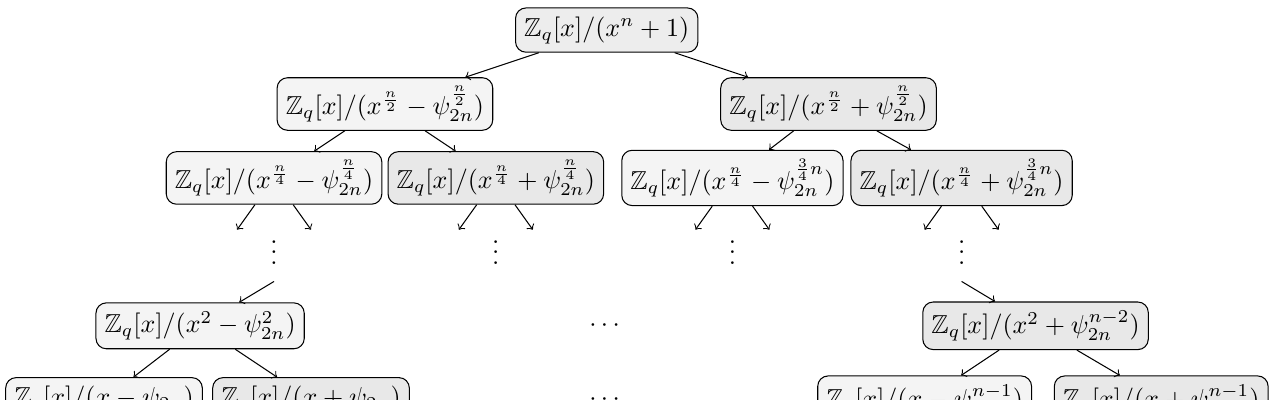
\includegraphics[width=0.90\textwidth,keepaspectratio]{imagenes/autores_cap2/fig_anillo_reduccion_ciclotomica.png}
	\caption{Descomposición y reducción ciclotómica en el anillo polinomial $\mathbb{Z}_q[x]/(x^n + 1)$ mediante transformada NTT.}
	\label{fig:anillo_reduccion}
	\par\vspace{3pt}{\footnotesize\textit{ Liang y Zhao (2022), p. 12.}}
\end{figure}

Como muestra la Figura \ref{fig:anillo_reduccion}, la descomposición jerárquica del polinomio ciclotómico en factores lineales permite calcular multiplicaciones complejas en tiempo $\mathcal{O}(n \log n)$, logrando que un solo polinomio represente una fila completa de la matriz criptográfica y reduciendo drásticamente la cantidad de datos que deben transmitirse entre el navegador del votante y el servidor electoral.

\subsection{Module-LWE: El Compromiso Óptimo de FIPS 203 y 204}

Entre el problema LWE estándar (muy seguro pero con claves demasiado grandes) y el problema Ring-LWE (claves muy pequeñas pero con una estructura fija de un solo polinomio), existe un punto intermedio ideal que fue seleccionado por el NIST para sus estándares oficiales: el problema de \textbf{Aprendizaje con Errores sobre Módulos} o Module-LWE (Langlois y Stehlé, 2015).

La idea de Module-LWE es muy clara: en lugar de usar matrices enormes de números sueltos y en lugar de usar un único polinomio aislado, se utiliza una matriz pequeña de tamaño $k \times k$ donde cada casilla contiene un polinomio de $256$ coeficientes:
\begin{equation}
	\mathbf{s} = \begin{pmatrix} s_1(x) \\ \vdots \\ s_k(x) \end{pmatrix} \in R_q^k, \quad \mathbf{A} \in R_q^{k \times k}
\end{equation}
De este modo, la ecuación con ruido mantiene exactamente la misma forma sencilla:
\begin{equation}
	\mathbf{b} = \mathbf{A} \cdot \mathbf{s} + \mathbf{e} \pmod q
\end{equation}
La gran ventaja de Module-LWE para la ingeniería de software es su flexibilidad. El grado del polinomio se mantiene siempre fijo en $n = 256$ (lo que permite reutilizar las mismas funciones rápidas de multiplicación NTT en el código fuente), y si se desea aumentar el nivel de seguridad del sistema, basta con cambiar el tamaño $k$ de la matriz (por ejemplo, usar $k = 2$ para seguridad básica, $k = 3$ para seguridad intermedia como en ML-KEM-768, o $k = 4$ para seguridad máxima). Con $k = 3$ y $n = 256$, el sistema opera sobre un retículo de $3 \times 256 = 768$ dimensiones utilizando claves compactas de apenas un kilobyte.

% =============================================================================
